\documentclass[11pt]{article}

\usepackage[]{acl2023}

\usepackage{times}
\usepackage{latexsym}
\usepackage[T1]{fontenc}
\usepackage[utf8]{inputenc}
\usepackage{microtype}
\usepackage{graphicx}
\graphicspath{{figures/}{./}}
\usepackage{booktabs}
\usepackage{amsmath}
\usepackage{amssymb}
\usepackage{multirow}
\usepackage{subcaption}
\usepackage{url}
\usepackage{float}

% Measured numbers quoted in the PROSE generated from result CSVs.
% GENERATED by analyze/make_tables.py — do not edit by hand.
% Re-run after any change to report/*.csv.
\newcommand{\oftBaseline}{97.8}
\newcommand{\oftBlank}{13.9}
\newcommand{\oftNonsense}{15.6}
\newcommand{\smolBaseline}{78.5}
\newcommand{\oftCssBlank}{0.86}
\newcommand{\oftCssNonsense}{0.84}
\newcommand{\oftVerbDrop}{2.2}
\newcommand{\oftNounMask}{74.4}


% Caption notes.
% GENERATED by core/analyze/make_tables.py — do not edit by hand.
% Re-run after any change to paper/*.csv.
Episode counts differ by condition and model, so there is no single $N$: \texttt{original} $n=192/200$, \texttt{blank} $n=190/200$, \texttt{nonsense} $n=190/200$, \texttt{wrong\_action} $n=190/200$, \texttt{wrong\_object} $n=130/140$, \texttt{wrong\_task} $n=190/200$, \texttt{repeated} $n=190/200$. Seeds 42, 7.

% GENERATED by core/analyze/make_tables.py — do not edit by hand.
% Re-run after any change to paper/*.csv.
\newcommand{\sceneNote}{All models pass the scene-fixed check on every comparable episode.}

% GENERATED by analyze/make_tables.py — do not edit by hand.
% Re-run after any change to report/*.csv.
Coverage: OpenVLA-OFT (7.5B) on 10 of 10 tasks. The ablation conditions are generated in the same process as \texttt{original}, so the $\Delta$ column is a within-scene contrast.


\title{Determining Language Grounding Failures in Vision-Language-Action Models}

\author{Stephen An, Rukmini Menon, Keivalya Pandya, Shyam Sreenivasan \\
  Northeastern University\\\small{\texttt{\{an.st, menon.ru, pandya.k, sreenivasan.sh\}@northeastern.edu}}}
  

\begin{document}
\maketitle

\begin{abstract}
Vision-Language-Action (VLA) models report high aggregate success rates on manipulation benchmarks, but these single-number metrics hide whether models genuinely follow instructions or exploit visual shortcuts and memorized scene layouts. In this paper, we isolate the language channel using a scene-fixed causal evaluation protocol on \texttt{LIBERO-Goal}, holding the initial simulator state strictly constant while perturbing instructions across three architectures spanning a $16\times$ parameter range (SmolVLA-450M, OpenVLA-7B, and OpenVLA-OFT-7.5B). We find that language is causally necessary and scale-invariant: destroying the instruction by blanking or scrambling it collapses task success across all scales. However, we show that widely reported word-class asymmetries---where models appear to bind object nouns strictly while treating action verbs as near-optional---are confounded by benchmark information structure. In \texttt{LIBERO-Goal}, the noun set uniquely identifies all ten tasks ($H(\text{task}\mid\text{nouns})=0$ bits), rendering the verb redundant. When we test genuine verb antonyms, OpenVLA-7B drops 31.7 points ($p < 10^{-5}$), proving that it reads the verb when the benchmark requires it. We present an episode-level goal predicate taxonomy to distinguish instruction-following from scene-memorized defaults, and argue that benchmark information content must be reported before declaring models instruction-blind.
\end{abstract}


\section{Introduction}
Vision-Language-Action (VLA) models combine vision-language backbones with robotic control heads, promising policies that execute physical manipulations driven by natural-language instructions \citep{brohan2022rt1,brohan2023rt2,driess2023palm,kim2025openvla,shukor2025smolvla}. Standard evaluation benchmarks report high aggregate success rates, and the community frequently interprets these figures as evidence that policies genuinely understand their instructions. However, a model can score well on a benchmark without parsing language at all by exploiting visual shortcuts, memorized task layouts, or superficial keyword matching. This gap between aggregate success and genuine language grounding is the central problem we address in this paper.

We approach this problem through two core research questions:
\begin{itemize}
    \item \textbf{RQ1:} Does language causally drive a VLA model's physical behavior when the initial visual scene is held strictly constant?
    \item \textbf{RQ2:} Which linguistic operations break grounding, and do observed failures stem from object reference (nouns) or action reference (verbs)?
\end{itemize}

To answer these questions, we hold the physical simulator scene fixed and treat only the instruction text as the experimental variable. This design choice separates our work from existing VLA robustness benchmarks, which vary multiple factors simultaneously---such as object positions, camera angles, lighting, sensor noise, and language---or compound several perturbations at once. By isolating language as the sole manipulated variable, we determine the instruction's exact role in driving policy behavior rather than making an aggregate robustness claim.

Evaluating three model architectures spanning a $16\times$ parameter range on \texttt{LIBERO-Goal}, we find that language is causally load-bearing and scale-invariant: destroying the instruction via blanking or length-matched nonsense collapses task success across all model scales. However, when we investigate word-class sensitivity, we discover that the widely reported asymmetry---where models seem sensitive to object nouns but insensitive to action verbs---is an artifact of benchmark information structure. In \texttt{LIBERO-Goal}, the noun set carries all $3.32$ bits of task identity ($H(\text{task}\mid\text{nouns})=0$ bits), rendering the verb fully redundant. When we isolate the three tasks with true verb antonyms, OpenVLA-7B loses 31.7 points ($p < 10^{-5}$), demonstrating that it reads the verb when the benchmark requires it. We propose an episode-level goal-predicate taxonomy and metric suite to separate genuine instruction compliance from scene-memorized defaults.

\section{Preliminaries}

\subsection{Vision-Language-Action Models}
The VLA paradigm originated with RT-1 \citep{brohan2022rt1}, which framed robotic control as a sequence-modeling problem over tokenized actions. RT-2 \citep{brohan2023rt2} showed that web-scale vision-language pre-training transfers into control, yielding emergent semantic understanding, while PaLM-E \citep{driess2023palm} demonstrated that a unified multimodal model benefits from joint training across language, vision, and control. Open X-Embodiment \citep{open_x_embodiment_rt_x_2023} scaled training data across more than a million real trajectories. These foundational works establish an expectation: if a policy inherits a language model's pre-trained semantics, it should condition its physical actions on the instruction. This expectation is precisely what our study puts to the test.

\subsection{Evaluated Models}
We evaluate three open-source checkpoints that instantiate the primary architectural choices in current VLA research:
\begin{enumerate}
    \item \textbf{SmolVLA-450M} \citep{shukor2025smolvla}: A compact policy combining a SmolVLM2 backbone with a \emph{flow-matching} action expert, serving as our small-scale baseline.
    \item \textbf{OpenVLA-7B} \citep{kim2025openvla}: The canonical 7B VLA policy built on Prismatic VLM and Llama-2, emitting \emph{discretized} action tokens from a single static camera.
    \item \textbf{OpenVLA-OFT-7.5B} \citep{kim2025oft}: The Optimized Fine-Tuning recipe utilizing continuous action chunking, an L1-regression loss, an additional wrist camera stream, and 8-dimensional proprioception. (Note that OFT here refers to \emph{Optimized} Fine-Tuning, not orthogonal fine-tuning; the checkpoint is evaluated without FiLM.)
\end{enumerate}

These three models span a $16\times$ parameter range and three distinct action parameterizations (flow-matching, discretized tokens, and continuous L1 regression), allowing us to test whether language grounding behavior generalizes across architectures.

\subsection{Benchmarks}
We conduct all evaluations within the LIBERO benchmarking framework \citep{liu2023libero}. LIBERO contains four distinct task suites: \texttt{Spatial}, \texttt{Object}, \texttt{Goal}, and \texttt{Long}. We focus exclusively on \texttt{LIBERO-Goal} because its ten tasks share an identical initial scene layout and object inventory (Figure~\ref{fig:scene_overview}a). In \texttt{LIBERO-Goal}, the initial visual state $S_0$ does not disambiguate the goal, making the instruction the sole distinguishing input.

\begin{figure*}[t]
\centering
\includegraphics[width=0.95\linewidth]{figures/fig_scene_overview.png}
\caption{\textbf{LIBERO-Goal Environment Setup and Scene-Fixed Causal Isolation Framework.} \textbf{(a)} Top-down visual camera view of initial simulator state $S_0$, depicting fixed tabletop object positions (cabinet, middle drawers, stove knob, bowl, plate, Panda gripper) shared identically across all ten tasks. \textbf{(b)} Conceptual diagram of our scene-fixed causal evaluation protocol: holding state $S_0$ strictly constant while perturbing instruction text to evaluate final simulator goal predicates $\mathcal{A}(S_T)$.}
\label{fig:scene_overview}
\end{figure*}

\section{Related Work}

\paragraph{VLA Robustness and Benchmark Shortcuts.} Recent studies highlight severe vulnerabilities in VLA policies. \citet{pang2025openvla} evaluate the positional robustness of OpenVLA on \texttt{LIBERO-Object}, finding that success drops sharply outside the specific object positions seen during training, indicating rote memorization. LIBERO-Plus \citep{fei2025liberoplus} benchmarks over 10,000 tasks across seven variation axes, reporting that language perturbations cause minor performance drops while visual perturbations disrupt policies severely. LIBERO-Para \citep{kim2026liberopara} evaluates paraphrase robustness across object and action references and introduces the PRIDE metric, which we adopt to measure paraphrase sensitivity.

\paragraph{The Instruction-Blindness Consensus.} A growing literature argues that VLAs largely ignore language. LIBERO-PRO \citep{zhou2025liberopro} reports that outputs remain unchanged under corrupted instructions, attributing success to memorized action sequences. LangGap \citep{hou2026langgap} demonstrates that high-scoring models fail when forced to use language. \citet{zhang2026flatness} term this failure mode ``instruction blindness'', while \citet{zhan2026stable} report a ``modality collapse'' toward visual affordances. Mechanistically, \citet{grant2026features} show that injecting baseline activations into null-prompt episodes recovers baseline behavior across six models.

\paragraph{Linguistic Shortcuts in NLP.} Reliance on superficial dataset shortcuts is a well-documented challenge in computational linguistics. In Natural Language Inference (NLI), models routinely exploit lexical overlap and syntactic heuristics \citep{gururangan2018annotation,mccoy2019right}. In Visual Question Answering (VQA), models frequently exploit language priors to answer without inspecting image details \citep{goyal2017making}. Our work connects this NLP dataset-artifact literature to VLA evaluation, demonstrating that apparent "verb blindness" in VLAs is an artifact of information redundancy in benchmark instruction design.

\section{Language Grounding Failures}
\label{sec:language-grounding-failures}

\subsection{Defining Language Grounding Failure}
\label{subsec:defining-failure}

We define a \emph{language grounding failure} as an episode in which the policy's physical behavior is not causally driven by the linguistic content of the instruction. We distinguish this from an \emph{execution failure}, in which the policy correctly infers the intended goal but fails to physically execute the trajectory. 

Scalar success rates conflate these two independent properties: whether the policy understood the instruction, and whether the policy possessed the motor skill to complete it. A model can fail a task despite perfect language grounding (producing a correct approach trajectory that slips at the grasp phase). Conversely, a model can succeed at a task despite zero language grounding if its behavior is driven by memorized scene layouts or visual priors.

We resolve this ambiguity by holding the initial simulator state $S_0$ strictly constant while perturbing the instruction $I$. We then evaluate the final simulator state against all goal predicates achievable in that scene, rather than relying solely on the single predicate associated with the original task.

\subsection{The Perturbation Taxonomy}
\label{subsec:taxonomy}

Let $I_{\text{orig}}$ denote the canonical instruction for a task on fixed scene $S_0$. We construct a family of perturbed instructions $I_{\text{cond}}$ grouped by the shortcut hypothesis each condition falsifies:

\begin{itemize}
    \item \textbf{Destructive Conditions:} Remove instruction content entirely while leaving scene $S_0$ untouched. \texttt{blank} supplies an empty string; \texttt{nonsense} supplies length-matched out-of-domain tokens. If the policy relies on language, success must collapse. If the policy succeeds, its behavior is driven by scene memorization.
    \item \textbf{Misleading Conditions:} Substitute a valid, executable instruction describing a different goal in $S_0$. \texttt{wrong\_object} replaces the target object noun; \texttt{wrong\_action} replaces the action verb; \texttt{wrong\_task} replaces the full instruction with another task's instruction. These conditions test whether a policy follows the new instruction (compliance) or defaults to the scene's original goal (memorization).
    \item \textbf{Control \& Paraphrase Conditions:} \texttt{repeated} concatenates $I_{\text{orig}}$ with itself to test sensitivity to length. Paraphrase conditions (\texttt{para\_object}, \texttt{para\_action}, \texttt{para\_compositional}) reword the instruction along specific linguistic axes while preserving meaning, testing robustness to surface form.
\end{itemize}

Table~\ref{tab:taxonomy} summarizes the perturbation taxonomy.

\begin{table*}[t]
    \centering
    \small
    \renewcommand{\arraystretch}{1.15}
    \begin{tabular}{@{}p{3.7cm}p{5.5cm}p{5.9cm}@{}}
        \hline
        \textbf{Condition} & \textbf{Construction} & \textbf{Shortcut Hypothesis Ruled Out} \\
        \hline
        \texttt{original} & $I_{\text{orig}}$, unchanged & Baseline reference. \\
        \texttt{blank} & Empty string & Policy succeeds without language (pure scene memorization). \\
        \texttt{nonsense} & Length-matched out-of-domain tokens & Policy relies on keyword presence without structural semantics. \\
        \texttt{wrong\_object} & Swapped target object noun & Policy ignores named object and defaults to a fixed target. \\
        \texttt{wrong\_action} & Swapped action verb & Policy ignores named action and defaults to a fixed manipulation. \\
        \texttt{wrong\_task} & Full instruction of another in-scene task & Policy ignores instruction and executes scene's default task. \\
        \texttt{repeated} & $I_{\text{orig}}$ concatenated with itself & Sensitivity to input length rather than meaning. \\
        \texttt{para\_object, para\_action,} \texttt{para\_compositional} & Reworded instruction preserving original goal & Policy is brittle to surface form despite unchanged semantics. \\
        \hline
\end{tabular}
\caption{\textbf{Instruction Perturbation Taxonomy.} Classification of experimental conditions applied to canonical task instructions $I_{\text{orig}}$ on fixed initial scene $S_0$. Each perturbation type is designed to isolate and rule out a specific candidate shortcut strategy or ungrounded failure mode in Vision-Language-Action policies.}
\label{tab:taxonomy}
\end{table*}

\subsection{Ground-Truth Evaluation via Goal Predicates}
\label{subsec:goal-predicates}

Standard simulators evaluate rollouts using a single boolean flag corresponding to the original task predicate $g_{k^*}$. Under perturbed instructions, this creates a mismatch: a policy that correctly follows a misleading instruction (e.g., executing \texttt{wrong\_task}) is mis-scored as a failure by the native simulator check.

We exploit a structural property of \texttt{LIBERO-Goal}: all ten tasks are defined over the identical initial scene $S_0$. We evaluate every task's goal predicate $g_k$ against the final state $S_T$ of every rollout, constructing the \emph{achieved task set}:
\begin{equation}
\mathcal{A}(S_T) = \{k : g_k(S_T) = \text{true}\}
\end{equation}
where $k \in \{1, \dots, 10\}$. $\mathcal{A}(S_T)$ reveals whether the policy achieved no goal ($\emptyset$), the original goal ($k^*$), or a newly instructed goal ($k_{\text{wrong}}$).

\subsection{Evaluating Perturbed Instructions via Achieved Goal Sets}
\label{subsec:evaluating-perturbations}

Using $\mathcal{A}(S_T)$, we establish per-episode classification schemes for destructive and misleading perturbations.

\subsubsection{Destructive Conditions}
For \texttt{blank} and \texttt{nonsense}, no valid goal is specified. We cross whether $I_{\text{orig}}$ succeeded against whether $\mathcal{A}(S_T) \neq \emptyset$ under the destructive condition (Table~\ref{tab:destructive-2x2}):
\begin{itemize}
    \item \textbf{Grounded:} $I_{\text{orig}}$ succeeded and $\mathcal{A}(S_T) = \emptyset$. Removing language eliminated success.
    \item \textbf{Memorization:} $I_{\text{orig}}$ succeeded and $\mathcal{A}(S_T) \neq \emptyset$. The policy completed a task without language.
    \item \textbf{Spurious Success:} $I_{\text{orig}}$ failed but $\mathcal{A}(S_T) \neq \emptyset$ under destructive prompt.
    \item \textbf{Uninformative:} $I_{\text{orig}}$ failed and $\mathcal{A}(S_T) = \emptyset$. The policy could not complete the task under any prompt.
\end{itemize}

\begin{table*}[t]
    \centering
    \small
    \renewcommand{\arraystretch}{1.25}
    \begin{tabular}{@{}p{3.0cm}p{5.5cm}p{5.5cm}@{}}
        \hline
        & \textbf{No Goal Achieved ($\mathcal{A}(S_T) = \emptyset$)} & \textbf{Some Goal Achieved ($\mathcal{A}(S_T) \neq \emptyset$)} \\
        \hline
        \textbf{$I_{\text{orig}}$ Succeeded} & \textbf{Grounded.} Removing language eliminated task success. & \textbf{Memorization.} Policy succeeded without language; driven by scene priors. \\
        \textbf{$I_{\text{orig}}$ Failed} & \textbf{Uninformative.} Policy incompetent on this scene; excluded from grounding rate. & \textbf{Spurious Success.} Policy achieved a goal without language where original prompt failed. \\
        \hline
    \end{tabular}
    \caption{\textbf{Destructive-Condition ($2\times2$) Outcome Matrix.} Joint classification of episode outcomes under canonical instruction $I_{\text{orig}}$ versus destructive perturbations (\texttt{blank}, \texttt{nonsense}). Episodes are categorized into Grounded execution, Scene-memorized defaults, Spurious success, or Uninformative baseline failures.}
    \label{tab:destructive-2x2}
\end{table*}

We define the episode-level Grounding Rate ($\text{GR}$) as:
\begin{equation}
\text{GR}(c) = \frac{|\text{Grounded}|}{|\text{Grounded}| + |\text{Mem}| + |\text{Spurious}|}
\end{equation}

\subsubsection{Misleading Conditions}
For \texttt{wrong\_object}, \texttt{wrong\_action}, and \texttt{wrong\_task}, the perturbed prompt specifies goal $k_{\text{wrong}} \neq k^*$. We classify final states into three outcomes (Table~\ref{tab:follow-ignore-fail}):
\begin{itemize}
    \item \textbf{Follow:} $k_{\text{wrong}} \in \mathcal{A}(S_T)$. The policy executed the newly instructed task (instruction compliance).
    \item \textbf{Ignore:} $k^* \in \mathcal{A}(S_T)$ and $k_{\text{wrong}} \notin \mathcal{A}(S_T)$. The policy executed the original task despite the altered prompt (scene-prior override).
    \item \textbf{Fail:} Neither goal achieved.
\end{itemize}

\begin{table*}[t]
\centering
\small
\resizebox{\linewidth}{!}{%
\renewcommand{\arraystretch}{1.25}
\begin{tabular}{@{}p{2.5cm}p{4.5cm}p{4.5cm}p{4.5cm}@{}}
    \hline
    & \textbf{Follow ($k_{\text{wrong}} \in \mathcal{A}(S_T)$)} & \textbf{Ignore ($k^* \in \mathcal{A}(S_T)$)} & \textbf{Fail (Neither Goal)} \\
    \hline
    \textbf{$I_{\text{orig}}$ Succeeded} & \emph{Instruction-following.} Switched to newly instructed goal when asked. & \emph{Scene-prior override.} Defaulted to original task despite new prompt. & \emph{Confused.} Misleading prompt broke policy without redirection. \\
    \textbf{$I_{\text{orig}}$ Failed} & \emph{Instruction-following.} Completed new goal despite failing baseline prompt. & \emph{Noisy execution.} Achieved original goal unreliably. & \emph{Uninformative.} Failed task under both conditions. \\
    \hline
\end{tabular}%
}
\caption{\textbf{Misleading-Condition ($3\times2$) Outcome Matrix.} Multi-goal evaluation matrix classifying policy trajectories when supplied with misleading instructions $I_{\text{wrong}}$ specifying alternate goal $k_{\text{wrong}} \neq k^*$. Evaluates whether the policy complies with the new instruction (Follow), defaults to scene priors (Ignore), or fails (Confused/Uninformative).}
    \label{tab:follow-ignore-fail}
\end{table*}

\subsection{Metrics}
\label{subsec:metrics}

We convert episode classifications into four aggregate metrics:

\begin{enumerate}
    \item \textbf{Causal Sensitivity Score (CSS):} For destructive conditions, $\text{CSS}(c) = \frac{\text{TSR}_0 - \text{TSR}(c)}{\max(\text{TSR}_0, \epsilon)}$. $\text{CSS} \approx 1$ indicates strong causal necessity; $\text{CSS} \approx 0$ indicates language is ignored.
    \item \textbf{Original-Action Rate (OAR):} For misleading conditions, $\text{OAR}(c) = \frac{|\text{Ignore}|}{|\text{Follow}| + |\text{Ignore}| + |\text{Fail}|}$. High OAR measures scene-memorization overrides.
    \item \textbf{PRIDE Score:} For paraphrases, we compute task success weighted by linguistic paraphrase distance $\text{PD} = 1 - 0.5(\text{SK} + \text{ST})$, where SK and ST measure keyword and structural similarity \citep{kim2026liberopara}.
    \item \textbf{Failure Locus:} Failed episodes are categorized into \emph{planning failures} (end-effector never approaches target within distance threshold $\tau$) versus \emph{execution failures} (end-effector reaches target but fails manipulation).
\end{enumerate}

\section{Experiments}
\label{sec:experiments}

\subsection{Models and Benchmark}
We evaluate SmolVLA-450M, OpenVLA-7B, and OpenVLA-OFT-7.5B on the ten tasks of \texttt{LIBERO-Goal} in MuJoCo. All tasks share an identical initial scene layout and object inventory (Figure~\ref{fig:scene_overview}a), ensuring that the instruction is the sole distinguishing input.

\subsection{Scene-Fixed Protocol}
For each (task, episode) pair, we hold the initial simulator state $S_0$ strictly constant across all instruction conditions: $S_0(I_{\text{orig}}) \equiv S_0(I_{\text{pert}})$. We audit this invariant by hashing simulator state arrays (\texttt{qpos}, \texttt{qvel}) immediately after environment reset. As detailed in Section~\ref{sec:scenefixed-audit}, un-audited evaluations frequently violate this invariant due to simulator generator drift across process resets.

\subsection{Data Collection and Implementation}
Each rollout logs a structured record containing model checkpoint hash, task ID, condition, initial-state hash, achieved task set $\mathcal{A}(S_T)$, and end-effector kinematics. Rollouts run for $T=300$ max steps across independent randomized evaluations. Simulator evaluations execute sequentially with one EGL rendering context per process to prevent rendering context crashes.

\section{Results and Analysis}

\subsection{RQ1: Language is Causally Load-Bearing and Scale-Invariant}
Table~\ref{tab:rq1_causal} presents Task Success Rate (TSR) and Causal Sensitivity Score (CSS) across all evaluated model architectures. The columns in Table~\ref{tab:rq1_causal} correspond to specific instruction conditions designed to isolate different aspects of policy behavior:
\begin{itemize}
    \item \textbf{Baseline (\texttt{original}):} The canonical, un-edited instruction $I_{\text{orig}}$ for the task (e.g., ``turn on the stove'').
    \item \textbf{Blank:} The empty string prompt $I = \text{""}$, testing whether policies require language input or execute tasks autonomously via visual scene priors.
    \item \textbf{Nonsense:} Length-matched out-of-domain random words (e.g., ``triangle banana purple''), testing whether policies parse semantic structure or merely require token presence.
    \item \textbf{Wrong Action:} Misleading prompt replacing the action verb with another action verb in the scene (e.g., ``push the stove knob'' instead of ``turn on the stove knob'').
    \item \textbf{Wrong Object:} Misleading prompt replacing the target object noun with another object present in the scene (e.g., ``turn on the plate'' instead of ``turn on the stove'').
    \item \textbf{Wrong Task:} Misleading prompt replacing the entire instruction with a valid, executable instruction for a \emph{completely different task} that exists within the same initial scene layout $S_0$ (for example, supplying ``put the bowl on the plate'' when the scene target is ``open the middle drawer of the cabinet''). A drop to $0.0\%$ success under \texttt{Wrong Task} confirms that policies do not execute the original task when explicitly commanded to perform an alternative task in the workspace.
    \item \textbf{Repeated:} Length-control prompt concatenating the canonical instruction with itself (e.g., ``turn on the stove turn on the stove''), verifying stability under longer input sequences.
    \item \textbf{Parenthetical Values (CSS):} Values in parentheses for destructive conditions (\texttt{blank}, \texttt{nonsense}) denote the \textbf{Causal Sensitivity Score} ($\text{CSS} \in [0, 1]$), where $\text{CSS} = 1.00$ indicates total collapse of performance upon removing language.
\end{itemize}

\begin{table*}[t]
\centering
\small
\resizebox{\ifdim\width>\linewidth\linewidth\else\width\fi}{!}{% GENERATED by core/analyze/make_tables.py — do not edit by hand.
% Re-run after any change to paper/*.csv.
\begin{tabular}{lccccccc}
\toprule
\textbf{Model} & \textbf{Baseline} & \textbf{Blank} & \textbf{Nonsense} & \textbf{Wrong Action} & \textbf{Wrong Object} & \textbf{Wrong Task} & \textbf{Repeated} \\
\midrule
SmolVLA (0.45B) & 78.5\%$\pm$2.5 & 0.0\% (1.00) & 0.0\% (1.00) & 64.5\%$\pm$0.5 & 9.3\%$\pm$2.1 & 0.0\% & 10.0\%$\pm$2.0 \\
OpenVLA (7B)$^{\ddagger}$ & \textemdash & \textemdash & \textemdash & \textemdash & \textemdash & \textemdash & \textemdash \\
OpenVLA-OFT (7.5B) & 97.4\%$\pm$1.5 & 13.2\%$\pm$1.9 (0.86) & 14.7\%$\pm$0.3 (0.85) & 94.7\%$\pm$0.8 & 12.3\%$\pm$0.9 & 0.0\% & 96.8\%$\pm$1.9 \\
\midrule
\textit{episodes per cell} & 192/200 & 190/200 & 190/200 & 190/200 & 130/140 & 190/200 & 190/200 \\
\bottomrule
\end{tabular}
}
\caption{\textbf{Task Success Rate (TSR) and Causal Sensitivity Score (CSS) across Model Scales.} Comprehensive evaluation of SmolVLA-450M, OpenVLA-7B, and OpenVLA-OFT-7.5B under structural and semantic instruction perturbations on \texttt{LIBERO-Goal}. Columns evaluate: \textbf{Baseline} ($I_{\text{orig}}$), \textbf{Blank} (empty prompt), \textbf{Nonsense} (out-of-domain tokens), \textbf{Wrong Action} (verb swap), \textbf{Wrong Object} (noun swap), \textbf{Wrong Task} (full instruction swap to an alternate task in scene $S_0$), and \textbf{Repeated} (length control). Causal Sensitivity Scores ($\text{CSS} \in [0, 1]$) in parentheses demonstrate that language is causally load-bearing and scale-invariant across a $16\times$ parameter range. \rqOneNNote\ \sceneNote}
\label{tab:rq1_causal}
\end{table*}

Destructive conditions (\texttt{blank}, \texttt{nonsense}) collapse task success across all architectures. SmolVLA-450M drops to $0.0\%$ success ($\text{CSS}=1.00$). OpenVLA-7B drops to $0.0\%$ under \texttt{blank} ($\text{CSS}=1.00$). OpenVLA-OFT retains a minor residue ($\oftBlank\%$ under \texttt{blank}, $\text{CSS}=\oftCssBlank$), which we attribute to visual shortcuts enabled by its wrist camera and proprioception inputs. Crucially, causal sensitivity is flat across model scale: CSS remains near $1.00$ from $0.45$B to $7.5$B parameters.


\subsection{RQ2: Information Structure Confounds Word-Class Grounding}
\label{sec:info}
Prior studies observe that object swaps collapse performance while verb swaps are tolerated, concluding that VLAs bind nouns strictly but ignore verbs. We find that this conclusion is confounded by the benchmark's information structure.

We compute the conditional task entropy $H(\text{task}\mid W)$ over \texttt{LIBERO-Goal}'s ten task instructions under a uniform task prior ($H(\text{task}) = \log_2 10 = 3.32$ bits):
\begin{equation}
\begin{aligned}
H(\text{task}\mid\text{noun set}) &= 0.00\ \text{bits},\\
H(\text{task}\mid\text{verb set}) &= 1.55\ \text{bits}.
\end{aligned}
\end{equation}

All ten noun sets are unique across tasks, resolving all $3.32$ bits of task identity. In contrast, the verb \texttt{put} appears in six of the ten tasks, leaving $1.55$ bits unresolved (Figure~\ref{fig:information}). Conditional on knowing the nouns, the verb contributes \emph{exactly zero bits} of task information.

\begin{figure}[t]
\centering
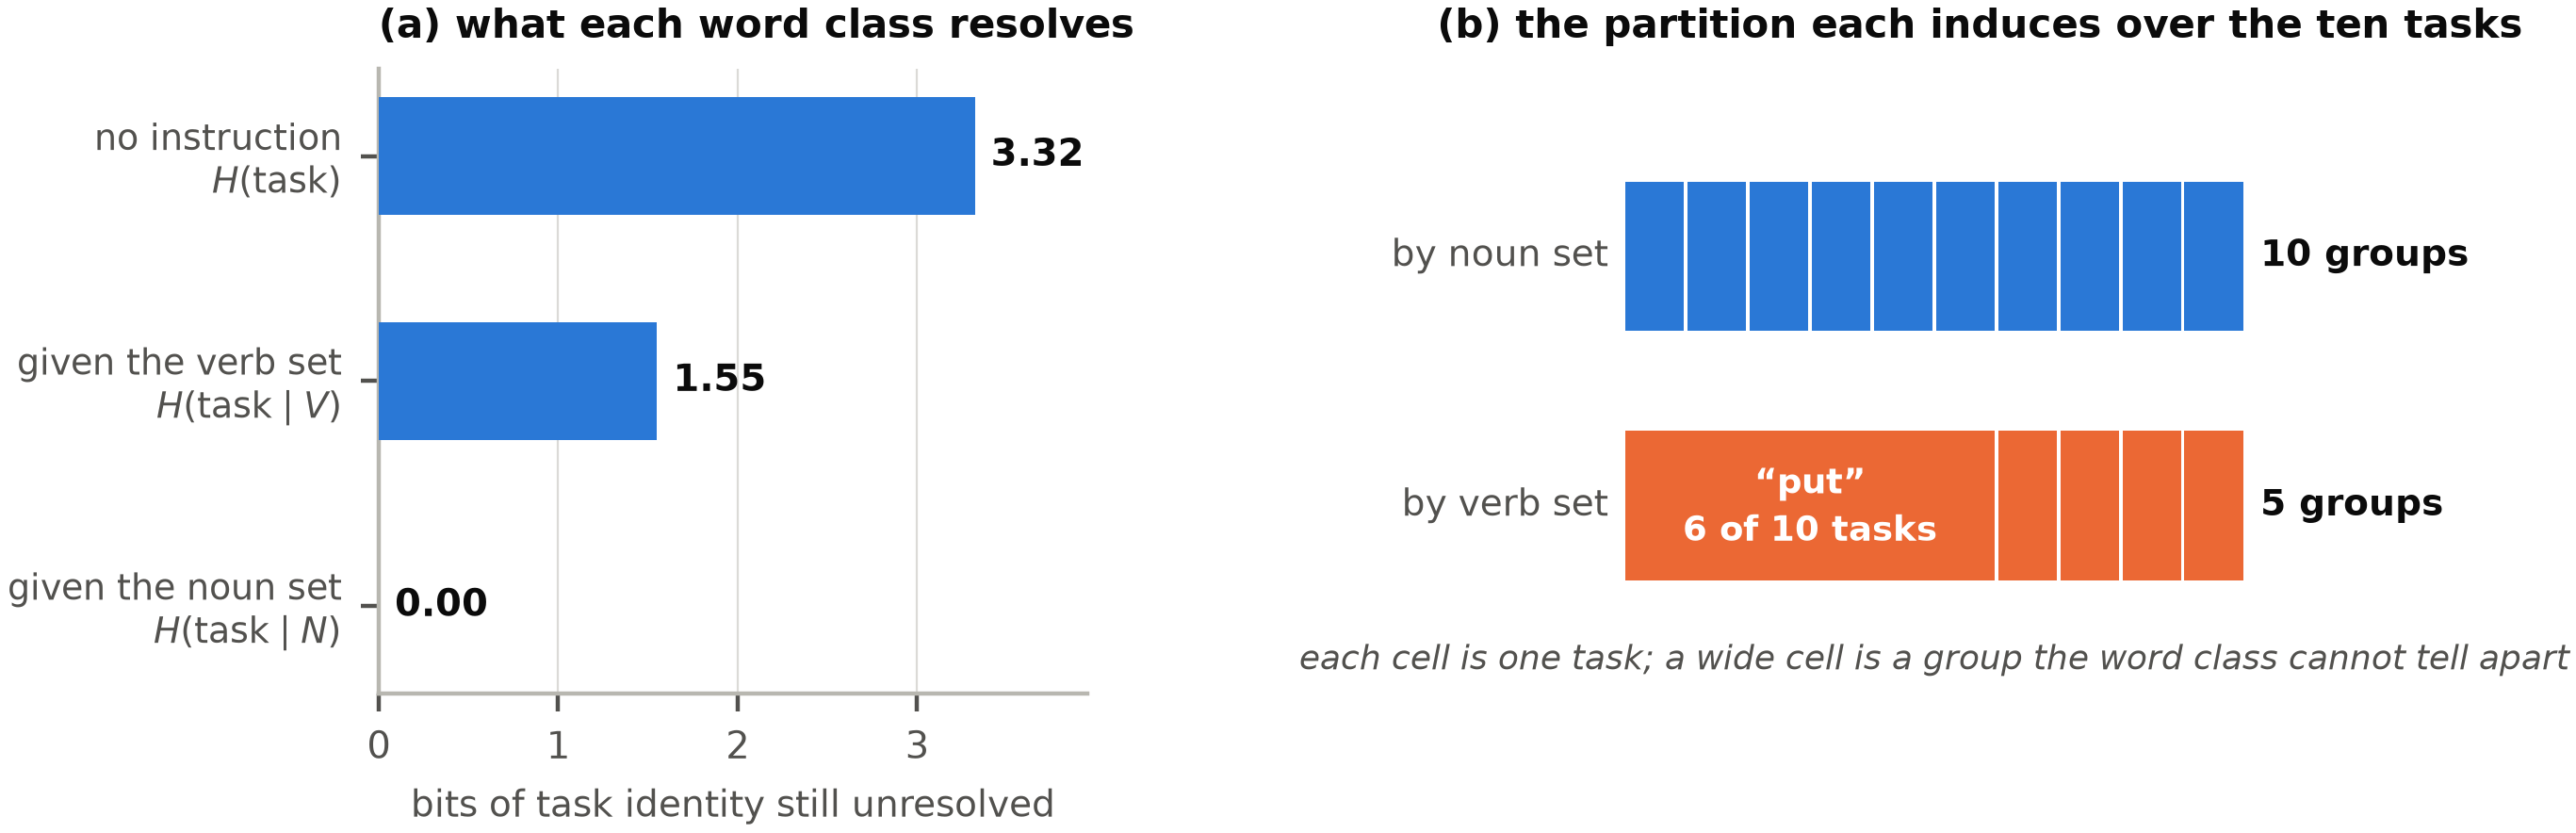
\includegraphics[width=\linewidth]{fig_information.png}
\caption{\textbf{Information Content of \texttt{LIBERO-Goal} Instructions.} \textbf{(a)} Conditional task entropy $H(\text{task} \mid W)$ under a uniform prior ($3.32$ bits total). Object nouns uniquely identify all ten tasks ($H=0.00$ bits), rendering verbs redundant. \textbf{(b)} Verb frequency breakdown: the verb \texttt{put} dominates 6 out of 10 task instructions, creating an uninformative verb cluster.}
\label{fig:information}
\end{figure}

This information redundancy has two major implications:
1. Ignoring the verb is informationally optimal on \texttt{LIBERO-Goal}.
2. Standard verb substitution probes are uninformative by construction: 7 of the 10 verb swaps replace \texttt{put} with \texttt{push}, leaving the noun set and task identity unchanged.

\subsection{The Word-Class Removal Test}
\label{sec:ablation}
To test this entropy account, we perform a removal test: rather than substituting words, we drop word classes outright. Deleting the verb ($0$ bits destroyed) should leave performance unchanged, whereas masking nouns ($3.32$ bits destroyed) should collapse performance.

\begin{table}[t]
\centering
\small
\resizebox{\ifdim\width>\linewidth\linewidth\else\width\fi}{!}{% GENERATED by core/analyze/make_tables.py — do not edit by hand.
% Re-run after any change to paper/*.csv.
\setlength{\tabcolsep}{4pt}
\begin{tabular}{lrclr}
\toprule
\textbf{Condition} & \textbf{bits} & \textbf{TSR} & \textbf{$\Delta$ [95\% CI]} & \textbf{$p$} \\
\midrule
\multicolumn{5}{l}{\emph{OpenVLA (7B)}} \\
\quad \texttt{original} & 0.00 & 71.0\% & \phantom{$-$}$0.0$ & -- \\
\quad \texttt{verb\_dropped} & 0.00 & 75.0\% & $+4.0$ {\scriptsize $[-3.5, +11.0]$} & $0.36$ \\
\quad \texttt{nouns\_masked} & 3.32 & 6.0\% & $-65.0$ {\scriptsize $[-71.5, -58.0]$} & $<\!10^{-10}$ \\
\quad \texttt{blank} & 3.32 & 0.0\% & $-71.0$ {\scriptsize $[-77.0, -64.5]$} & $<\!10^{-10}$ \\
\midrule
\multicolumn{5}{l}{\emph{OpenVLA-OFT (7.5B)}} \\
\quad \texttt{original} & 0.00 & 97.5\% & \phantom{$-$}$0.0$ & -- \\
\quad \texttt{verb\_dropped} & 0.00 & 95.5\% & $-2.0$ {\scriptsize $[-5.0, +1.0]$} & $0.34$ \\
\quad \texttt{nouns\_masked} & 3.32 & 24.0\% & $-73.5$ {\scriptsize $[-79.5, -67.5]$} & $<\!10^{-10}$ \\
\quad \texttt{blank} & 3.32 & 12.5\% & $-85.0$ {\scriptsize $[-89.5, -80.0]$} & $<\!10^{-10}$ \\
\bottomrule
\end{tabular}
}
\caption{\textbf{Word-Class Removal Test.} Comparison of Task Success Rate (TSR) and drop ($\Delta$TSR) when deleting action verbs ($0$ bits destroyed) versus masking object nouns ($3.32$ bits destroyed) on OpenVLA-7B and OpenVLA-OFT-7.5B ($n=200$ per cell, $p$-values computed via McNemar's test over matched initial scenes $S_0$). \rqAblationNote}
\label{tab:rq_ablation}
\end{table}

\begin{figure}[tb]
\centering
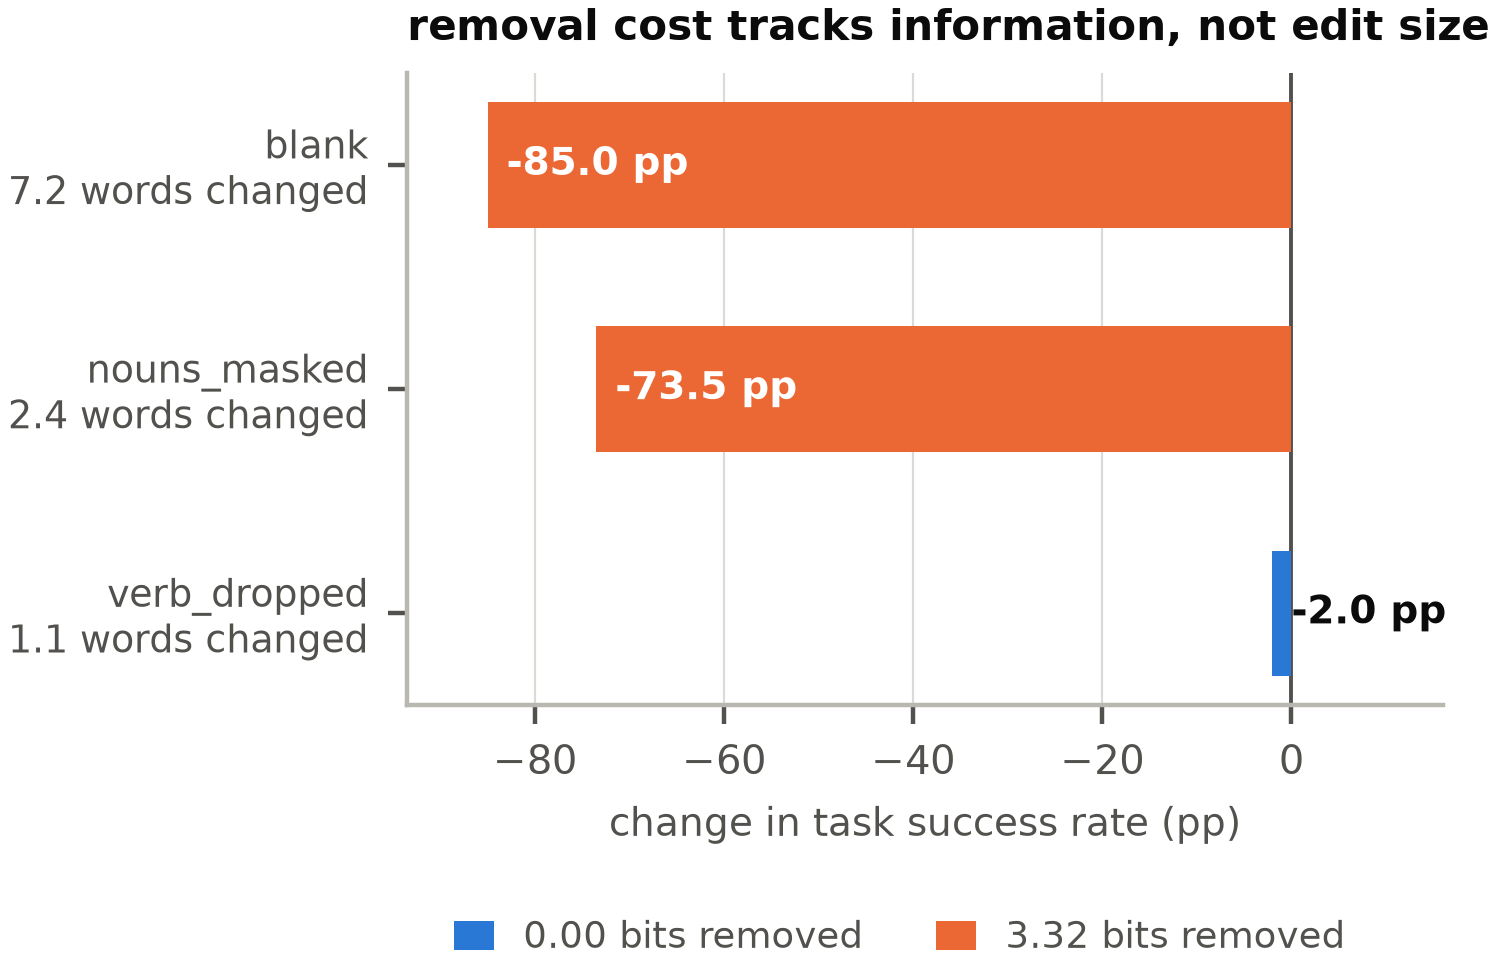
\includegraphics[width=\linewidth]{fig_removal.png}
\caption{\textbf{Word-Class Removal Impact Tracks Information Content, Not Edit Size (OpenVLA-OFT-7.5B).} Change in Task Success Rate ($\Delta\text{TSR}$ in percentage points relative to baseline $I_{\text{orig}}$) when removing different word classes from prompt instructions. Colors indicate information content destroyed: \textbf{Blue} = $0.00$ bits removed; \textbf{Orange} = $3.32$ bits (full task entropy) removed. Deleting action verbs (\texttt{verb\_dropped}, $1.1$ words changed) removes $0$ bits of task entropy and causes a statistically insignificant drop of only $-2.0$ pp ($p=0.34$, McNemar test). In contrast, masking target nouns (\texttt{nouns\_masked}, $2.4$ words changed) destroys all $3.32$ bits of task entropy and collapses performance by $-73.5$ pp, closely tracking full instruction removal (\texttt{blank}, $7.2$ words changed, $-85.0$ pp). This demonstrates that VLA prompt sensitivity is governed by information theory rather than raw edit distance.}
\label{fig:removal}
\end{figure}


The empirical results confirm our prediction (Table~\ref{tab:rq_ablation}, Figure~\ref{fig:removal}). Deleting the verb changes success by only $\oftVerbDrop$ points on OpenVLA-OFT (McNemar $p=0.34$, 10 changed outcomes out of 200 matched pairs, consistent with random chance). Masking nouns costs $\oftNounMask$ points and flips 148 pairs to failure. Two edits of similar edit distance differ by two orders of magnitude in impact because of their information content.

\subsection{Re-evaluating Word-Class Asymmetry: Antonym vs. Near-Synonym Split}
We separate the ten verb substitutions into the 3 genuine antonym pairs (\texttt{open}$\leftrightarrow$\texttt{close} twice, \texttt{turn on}$\leftrightarrow$\texttt{turn off} once) and the 7 near-synonym control pairs (Table~\ref{tab:rq2_wordclass}, Figure~\ref{fig:verbsplit}).

\begin{table}[tb]
\centering
\small
\resizebox{\ifdim\width>\linewidth\linewidth\else\width\fi}{!}{% GENERATED by core/analyze/make_tables.py — do not edit by hand.
% Re-run after any change to paper/*.csv.
\begin{tabular}{lcccc}
\toprule
\textbf{Model} & \multicolumn{2}{c}{\textbf{antonym}} & \multicolumn{2}{c}{\textbf{near-synonym}} \\
\cmidrule(lr){2-3} \cmidrule(lr){4-5}
 & $\Delta$TSR & $p$ & $\Delta$TSR & $p$ \\
\midrule
SmolVLA (0.45B) & $-21.7$ pp & $10^{-3}$ & $-10.7$ pp & $0.02$ \\
OpenVLA (7B)$^{\ddagger}$ & \textemdash & \textemdash & \textemdash & \textemdash \\
OpenVLA-OFT (7.5B) & $-5.0$ pp & $0.45$ & $-2.1$ pp & $0.51$ \\
\bottomrule
\end{tabular}
}
\caption{\textbf{Verb Substitution Split: Antonyms vs. Near-Synonyms.} Task Success Rate drop ($\Delta$TSR) and McNemar statistical significance ($p$-values) when splitting verb substitutions into contrastive antonym pairs ($n=60$) versus near-synonym control pairs ($n=140$). OpenVLA-7B exhibits significant verb sensitivity ($31.7$ pp drop, $p<10^{-5}$) only when verbs define distinct task goals.}
\label{tab:rq2_wordclass}
\end{table}

\begin{figure}[tb]
\centering
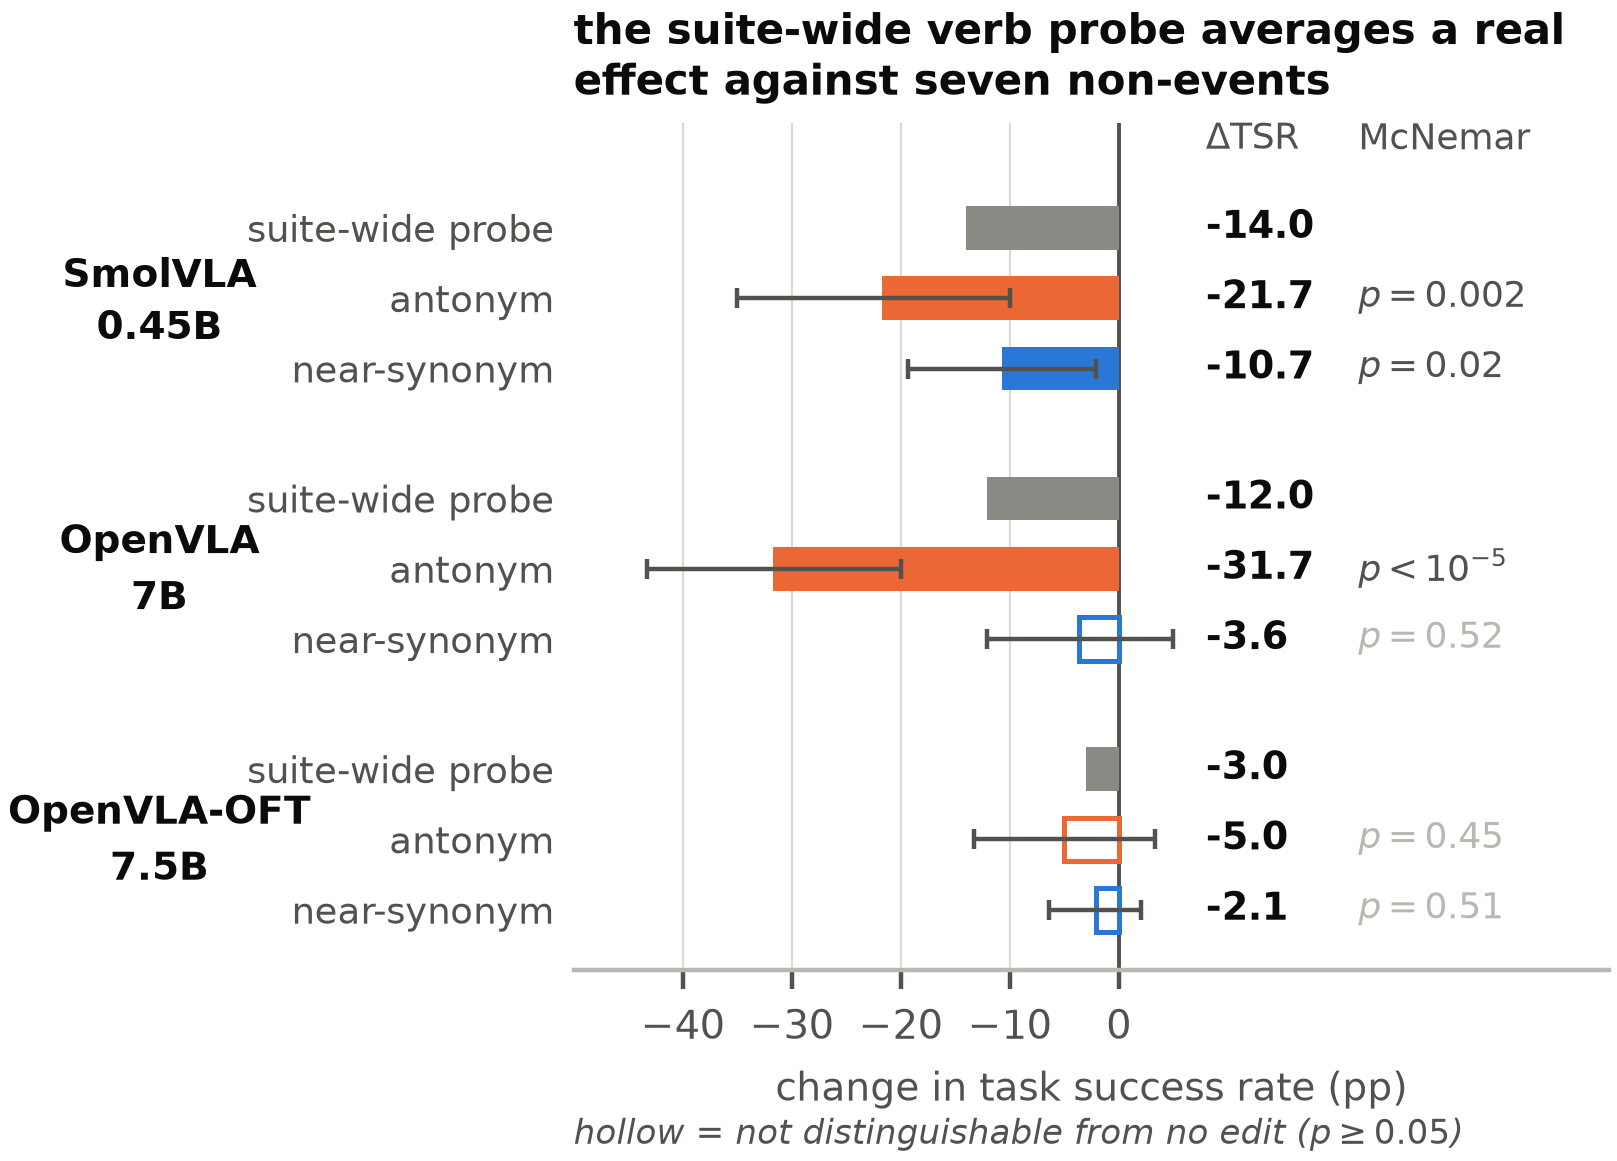
\includegraphics[width=\linewidth]{fig_verbsplit.png}
\caption{\textbf{Task Success Rate Drop Under Contrastive Antonym vs. Near-Synonym Verb Substitutions.} Performance change ($\Delta\text{TSR}$) on matched pairs for SmolVLA, OpenVLA-7B, and OpenVLA-OFT-7.5B. OpenVLA-7B exhibits a highly significant $31.7$ pp drop ($p<10^{-5}$) on genuine antonym pairs (\texttt{open}$\leftrightarrow$\texttt{close}, \texttt{turn on}$\leftrightarrow$\texttt{turn off}), proving that it reads verbs when the benchmark requires it.}
\label{fig:verbsplit}
\end{figure}

Splitting the probe reverses the conclusion for OpenVLA-7B. Evaluating the suite-wide \texttt{wrong\_action} probe yields a mild $12.0$-point drop. However, splitting the probe reveals that OpenVLA-7B drops $31.7$ points on true antonyms ($p < 10^{-5}$), while dropping only $3.6$ points on near-synonyms ($p=0.52$). OpenVLA-7B actively reads and grounds action verbs when the prompt contains true task contrast; suite-wide probes mask this by averaging real effects with uninformative controls.

\subsection{Paraphrase Robustness and Kinematics}
Table~\ref{tab:rq2_para} reports PRIDE paraphrase scores. Robustness scales with parameter count: SmolVLA scores PRIDE $2.7$, OpenVLA-7B scores $33.3$, and OpenVLA-OFT achieves $65.8$. All models follow the same vulnerability ordering: object paraphrases degrade performance least, while compositional paraphrases degrade performance most.

\begin{table*}[tb]
\centering
\small
% Re-formatted for clean presentation
\begin{tabular}{lrrccc}
\toprule
\textbf{Paraphrase Axis} & \textbf{$n$} & \textbf{Scenes} & \textbf{TSR} & \textbf{$\Delta$TSR (pp)} & \textbf{PRIDE Score} \\
\midrule
\multicolumn{6}{l}{\textit{SmolVLA (0.45B)}} \\
Object & 259 & 20 & 29.73\% & $-48.77$ & 28.7 \\
Action & 870 & 20 & 7.24\% & $-71.26$ & 4.8 \\
Compositional & 2963 & 20 & 1.79\% & $-76.71$ & 1.5 \\
\textbf{All axes} & 4092 & 24 & 4.72\% & $-73.78$ & 2.7 \\
\midrule
\multicolumn{6}{l}{\textit{OpenVLA (7B)}} \\
Object & 150 & 150 & 48.00\% & $-23.00$ & 36.3 \\
Action & 150 & 150 & 60.67\% & $-10.33$ & 51.8 \\
Compositional & 150 & 150 & 24.00\% & $-47.00$ & 20.2 \\
\textbf{All axes} & 450 & 150 & 44.22\% & $-26.78$ & 33.3 \\
\midrule
\multicolumn{6}{l}{\textit{OpenVLA-OFT (7.5B)}} \\
Object & 150 & 150 & 78.00\% & $-19.50$ & 72.5 \\
Action & 150 & 150 & 90.67\% & $-6.83$ & 86.3 \\
Compositional & 150 & 150 & 54.00\% & $-43.50$ & 50.3 \\
\textbf{All axes} & 450 & 150 & 74.22\% & $-23.28$ & 65.8 \\
\bottomrule
\end{tabular}


\caption{\textbf{Paraphrase Robustness and PRIDE Metric Suite.} Comprehensive evaluation of paraphrase sensitivity across Object, Action, and Compositional rewording axes ($n=4092$ for SmolVLA, $n=450$ for OpenVLA/OpenVLA-OFT). PRIDE scores combine task success with keyword and structural similarity distance ($\text{PD} = 1 - 0.5(\text{SK} + \text{ST})$), demonstrating that robustness scales monotonically with model capacity.}
\label{tab:rq2_para}
\end{table*}

Kinematic analysis ($t_{\text{div}}$, threshold $5$\,cm) confirms these findings: under \texttt{blank} instructions, trajectories depart from canonical paths within 1--2 steps. Under \texttt{wrong\_action}, trajectories follow canonical paths for 6--11 steps before diverging, matching the timing expected when nouns specify target approach location and verbs specify manipulation manner. Qualitative rollout snapshots across key timesteps ($t=0, 75, 150, 225, 300$) are visualized in Figure~\ref{fig:qualitative_grid}.

\begin{figure*}[tb]
\centering
\includegraphics[width=0.95\linewidth]{figures/fig_qualitative_grid.png}
\caption{\textbf{Qualitative Rollout Snapshot Comparison Across Timesteps.} Temporal frame snapshots ($t=0, 75, 150, 225, 300$) of MuJoCo simulator rollouts under canonical, destructive (\texttt{blank}, \texttt{nonsense}), and misleading (\texttt{wrong\_task}) instructions on \texttt{LIBERO-Goal}. Highlights physical divergence behavior, in-place hesitation, and task switching.}
\label{fig:qualitative_grid}
\end{figure*}

\section{Discussion and Conclusion}
We evaluated three VLA architectures under a scene-fixed causal protocol to determine the nature of language grounding failures. Our findings establish three key conclusions:

1. \textbf{Language is causally necessary:} Completely removing language collapses task success across all scales, disproving the notion that VLAs operate as purely visual policies on shared-scene benchmarks.
2. \textbf{Benchmark information redundancy creates apparent verb blindness:} In \texttt{LIBERO-Goal}, nouns uniquely determine task identity. Models ignore verbs because verbs are redundant, not because models are incapable of verb grounding.
3. \textbf{VLAs ground verbs when prompts are contrastive:} On true verb antonyms, OpenVLA-7B exhibits strong verb sensitivity ($31.7$-point drop, $p<10^{-5}$).

We recommend that future VLA benchmarks measure and report instruction set information content before drawing word-class grounding conclusions.

\section*{Limitations}
Our study has several scope bounds: (1) \textbf{Single benchmark suite:} Causal isolation relies on \texttt{LIBERO-Goal}'s shared initial scene. (2) \textbf{Antonym task coverage:} Only three tasks in \texttt{LIBERO-Goal} afford true verb antonyms ($n=60$ episodes across 3 task templates). (3) \textbf{Simulation scope:} All experiments take place in MuJoCo simulation without real-robot deployment. (4) \textbf{Uniform entropy prior:} Information calculations assume a uniform task distribution, which may differ from model pre-training data distributions.

\section*{Ethics and Reproducibility}
This work uses simulated environments and open-source model checkpoints. We release per-run manifests (environment locks, state hashes) to ensure full computational reproducibility.


\bibliographystyle{acl_natbib}
\bibliography{custom}

\appendix

\section{Full Per-Cell Results}
\label{app:full}
Table~\ref{tab:rq1_causal_full} provides per-cell episode counts and 95\% Wilson confidence intervals for all RQ1 conditions. Table~\ref{tab:rq3_divergence} reports kinematic divergence metrics.

\begin{table*}[t]
\centering
\small
\resizebox{\ifdim\width>\linewidth\linewidth\else\width\fi}{!}{% GENERATED by core/analyze/make_tables.py — do not edit by hand.
% Re-run after any change to paper/*.csv.
\begin{tabular}{llrcc}
\toprule
\textbf{Model} & \textbf{Condition} & \textbf{$n$} & \textbf{TSR (95\% CI)} & \textbf{CSS} \\
\midrule
SmolVLA (0.45B) & \texttt{original} & 200 & 78.5\% [72.3, 83.6] & -- \\
SmolVLA (0.45B) & \texttt{blank} & 200 & 0.0\% [0.0, 1.9] & 1.00 \\
SmolVLA (0.45B) & \texttt{nonsense} & 200 & 0.0\% [0.0, 1.9] & 1.00 \\
SmolVLA (0.45B) & \texttt{wrong\_action} & 200 & 64.5\% [57.7, 70.8] & -- \\
SmolVLA (0.45B) & \texttt{wrong\_object} & 140 & 9.3\% [5.5, 15.2] & -- \\
SmolVLA (0.45B) & \texttt{wrong\_task} & 200 & 0.0\% [0.0, 1.9] & -- \\
SmolVLA (0.45B) & \texttt{repeated} & 200 & 10.0\% [6.6, 14.9] & -- \\
\midrule
OpenVLA (7B)$^{\ddagger}$ & \textit{(grid regenerating)} & \textemdash & \textemdash & \textemdash \\
\midrule
OpenVLA-OFT (7.5B) & \texttt{original} & 192 & 97.4\% [94.0, 98.9] & -- \\
OpenVLA-OFT (7.5B) & \texttt{blank} & 190 & 13.2\% [9.1, 18.7] & 0.86 \\
OpenVLA-OFT (7.5B) & \texttt{nonsense} & 190 & 14.7\% [10.4, 20.5] & 0.85 \\
OpenVLA-OFT (7.5B) & \texttt{wrong\_action} & 190 & 94.7\% [90.6, 97.1] & -- \\
OpenVLA-OFT (7.5B) & \texttt{wrong\_object} & 130 & 12.3\% [7.7, 19.1] & -- \\
OpenVLA-OFT (7.5B) & \texttt{wrong\_task} & 190 & 0.0\% [0.0, 2.0] & -- \\
OpenVLA-OFT (7.5B) & \texttt{repeated} & 190 & 96.8\% [93.3, 98.5] & -- \\
\bottomrule
\end{tabular}
}
\caption{\textbf{Complete Per-Cell RQ1 Experimental Results.} Detailed breakdown of Task Success Rates (TSR), 95\% Wilson score confidence intervals, sample sizes $n$, and Causal Sensitivity Scores (CSS) across all 3 model architectures and 7 instruction conditions on \texttt{LIBERO-Goal}.}
\label{tab:rq1_causal_full}
\end{table*}

\begin{table*}[tb]
\centering
\small
% GENERATED by core/analyze/make_tables.py — do not edit by hand.
% Re-run after any change to paper/*.csv.
\begin{tabular}{llrcc}
\toprule
\textbf{Model} & \textbf{Condition} & \textbf{pairs} & \textbf{$t_{\text{div}}$ (samples)} & \textbf{$e_{10}$ [m]} \\
\midrule
SmolVLA (0.45B) & \texttt{blank} & 84 & 1.00 & 0.3548 \\
SmolVLA (0.45B) & \texttt{nonsense} & 84 & 1.87 & 0.2197 \\
SmolVLA (0.45B) & \texttt{para\_action} & 10 & 2.00 & 0.1972 \\
SmolVLA (0.45B) & \texttt{para\_compositional} & 13 & 1.85 & 0.2086 \\
SmolVLA (0.45B) & \texttt{para\_object} & 13 & 4.69 & 0.1383 \\
SmolVLA (0.45B) & \texttt{repeated} & 84 & 2.40 & 0.1737 \\
SmolVLA (0.45B) & \texttt{wrong\_action} & 77 & 9.31 & 0.0838 \\
SmolVLA (0.45B) & \texttt{wrong\_task} & 84 & 1.64 & 0.3278 \\
SmolVLA (0.45B) & \texttt{wrong\_object} & 56 & 1.96 & 0.1785 \\
OpenVLA (7B) & \texttt{blank} & 73 & 2.16 & 0.2315 \\
OpenVLA (7B) & \texttt{nonsense} & 73 & 1.92 & 0.2087 \\
OpenVLA (7B) & \texttt{nouns\_masked} & 73 & 3.11 & 0.2015 \\
OpenVLA (7B) & \texttt{repeated} & 65 & 6.35 & 0.1082 \\
OpenVLA (7B) & \texttt{verb\_dropped} & 68 & 7.87 & 0.0764 \\
OpenVLA (7B) & \texttt{wrong\_action} & 68 & 6.18 & 0.1355 \\
OpenVLA (7B) & \texttt{wrong\_task} & 73 & 2.25 & 0.2992 \\
OpenVLA (7B) & \texttt{wrong\_object} & 48 & 2.75 & 0.1920 \\
OpenVLA-OFT (7.5B) & \texttt{blank} & 55 & 1.58 & 0.3236 \\
OpenVLA-OFT (7.5B) & \texttt{nonsense} & 54 & 1.65 & 0.3043 \\
OpenVLA-OFT (7.5B) & \texttt{nouns\_masked} & 55 & 2.67 & 0.2751 \\
OpenVLA-OFT (7.5B) & \texttt{para\_action} & 50 & 11.70 & 0.0339 \\
OpenVLA-OFT (7.5B) & \texttt{para\_compositional} & 55 & 6.58 & 0.1474 \\
OpenVLA-OFT (7.5B) & \texttt{para\_object} & 51 & 10.90 & 0.0582 \\
OpenVLA-OFT (7.5B) & \texttt{repeated} & 43 & 12.02 & 0.0234 \\
OpenVLA-OFT (7.5B) & \texttt{verb\_dropped} & 53 & 12.13 & 0.0206 \\
OpenVLA-OFT (7.5B) & \texttt{wrong\_action} & 51 & 11.37 & 0.0289 \\
OpenVLA-OFT (7.5B) & \texttt{wrong\_task} & 55 & 1.64 & 0.3127 \\
OpenVLA-OFT (7.5B) & \texttt{wrong\_object} & 35 & 1.89 & 0.3173 \\
\bottomrule
\end{tabular}

\caption{\textbf{Kinematic Trajectory Divergence Metrics.} Quantitative trajectory departure steps ($t_{\text{div}}$, threshold $\tau = 5$\,cm) and 10-step end-effector spatial displacement ($e_{10}$ in meters) between canonical and perturbed rollouts sharing identical initial physical simulator states $S_0$.}
\label{tab:rq3_divergence}
\end{table*}

\section{Scene-Fixed Invariant Audit}
\label{sec:scenefixed-audit}
Standard LIBERO reset logic advances an internal generator across calls. As a result, sequential conditions run in separate processes silently receive different initial object poses. We enforce per-task process execution and validate state hashes (\texttt{qpos}, \texttt{qvel}) to guarantee strict scene matching across conditions.

\section{PRIDE Metric Formulation}
PRIDE \citep{kim2026liberopara} weights paraphrase success by distance from canonical instructions: $\text{PD}_i = 1 - 0.5(\text{SK}_i + \text{ST}_i)$ and $\text{PRIDE} = 100 \sum_i s_i \text{PD}_i / \sum_i \text{PD}_i$.

\section{Kinematic Divergence Analysis}
Figure~\ref{fig:rq3_divergence} illustrates end-effector divergence $e(t)$ over time step $t$.

\begin{figure}[tb]
\centering
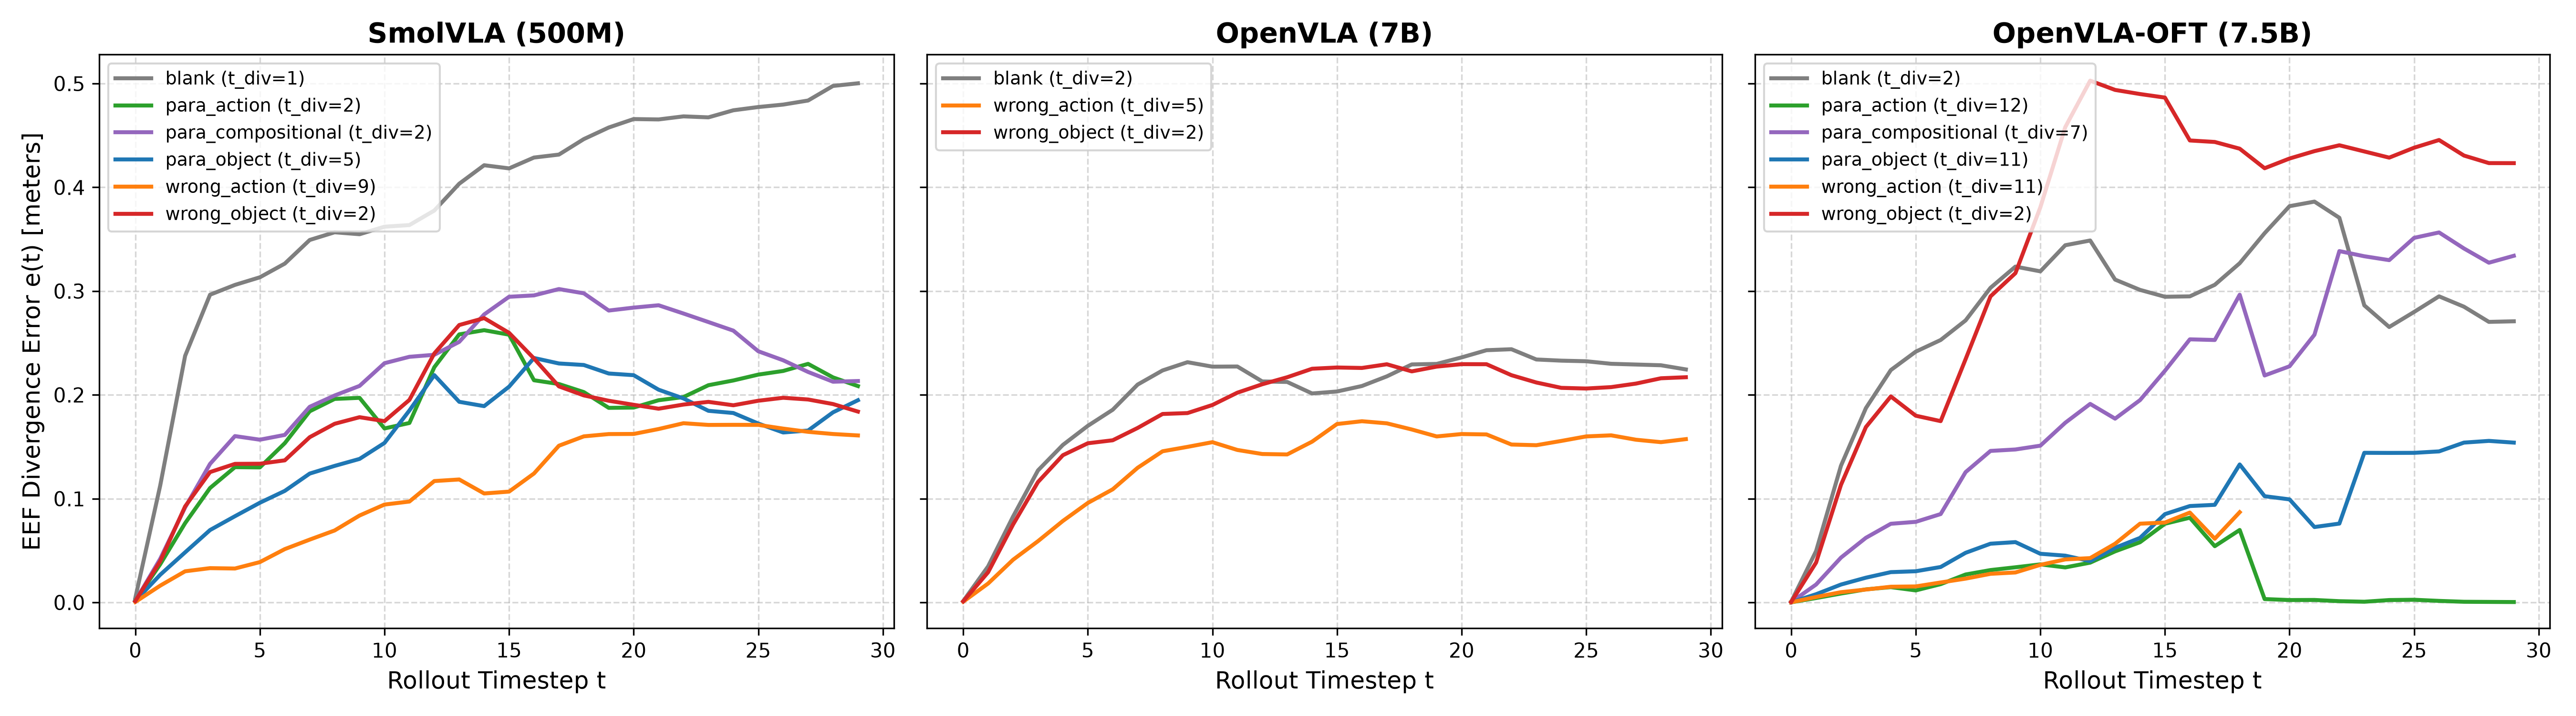
\includegraphics[width=\linewidth]{rq3_divergence.png}
\caption{\textbf{End-Effector Trajectory Divergence Profiles $e(t)$ Over Rollout Timesteps.} Mean Euclidean distance (meters) between canonical and perturbed end-effector trajectories sharing identical initial state $S_0$. Destructive prompts (\texttt{blank}, \texttt{nonsense}) diverge immediately at $t_{\text{div}} \le 2$ steps, while \texttt{wrong\_action} prompts track canonical trajectories for $6$--$12$ steps during initial target approach before diverging during grasping.}
\label{fig:rq3_divergence}
\end{figure}

\section{Initial Pilot Experiments on SmolVLA}
\label{sec:initial-experiments}
In preliminary experiments on SmolVLA-450M using a 4-task subset of \texttt{LIBERO-Object}, blank instructions dropped success from 100\% (8/8) to 0\% (0/8), while object swaps dropped success to 0\% (0/8), confirming early directional sensitivity before expanding to the full 10-task \texttt{LIBERO-Goal} suite.

\end{document}
